\section{Lecture 12: Liquid and Gaseous Analytic Rings, and the Tate Elliptic Curve}
\label{lec:12}

This lecture is a change of direction. So far the course has developed one
notion of completeness --- the solid theory (\cref{lec:5,lec:6}) and its
relative and Huber-pair variants (\cref{lec:7,lec:8,lec:9}) --- which is
well suited to nonarchimedean geometry and stays extremely close to Huber's
theory of adic spaces. Scholze now takes the broader view: completeness is not
to be fixed once and for all but is part of the datum of an \emph{analytic ring}
(\cref{lec:8}), and one would like many more examples, in particular ones that
accommodate archimedean geometry over $\mathbb{R}$ and $\mathbb{C}$, and ones
that combine the archimedean and nonarchimedean worlds. The organising example
is the \emph{Tate elliptic curve}. Following its coefficients leads to a Banach
ring $\mathbb{Z}(\!(q)\!)$ (with several natural norms), whose Berkovich
spectrum glues nonarchimedean and archimedean pieces; the question of putting an
analytic ring structure on it is answered by the \emph{liquid} theory, giving
$\alpha$-liquid structures on $\mathbb{R}$ and $\mathbb{Q}_p$; and the whole
family is organised by a single initial ``gaseous'' analytic ring, produced by
the course's new lightweight method of imposing endomorphisms of the projective
generator $P$.

Throughout, ``ring'' means commutative ring and everything lives in light
condensed abelian groups. We use freely the solid theory
$\Solid\subseteq\CondAbl$ (\cref{lec:5,lec:6}), the abstract notion of analytic
ring (\cref{lec:8}), and its localization over the adic/valuative spectrum
(\cref{lec:9,lec:10}).

\subsection{Where we are, and two questions}

\begin{remark}[Completeness as a relative notion]
\label{rmk:12:relative-completeness}
The point of departure was condensed mathematics as a framework for combining
homological algebra and functional analysis, in which one wanted a notion of
\emph{complete} module. The solid modules over $\mathbb{Z}$, over any finite type
$\mathbb{Z}$-algebra $R$ (\cref{lec:11}), and over any Huber pair gave one such
notion, closely tied to Huber's adic spaces. The conceptual lesson was that
completeness should not be an absolute notion fixed once and for all, but a
\emph{relative} one: it is part of the datum of what an analytic ring is,
namely the choice of which modules count as complete (\cref{def:8:analytic-ring}).
The programme is then to take analytic rings as building blocks and glue them,
as one glues affine schemes into schemes, to obtain analytic spaces --- and
within that world to locate the various classical notions of analytic space.
\end{remark}

Before building the general gluing formalism, one wants more examples of
analytic rings, and in particular a theory that is not only nonarchimedean.
This raises two questions, which will organise the lecture.

\begin{remark}[Two questions]
\label{rmk:12:two-questions}
\begin{enumerate}
\item Does $\mathbb{R}$ carry a natural analytic ring structure, suitable for
real and complex geometry?
\item Is there a good way to \emph{combine} the nonarchimedean and archimedean
theories into one?
\end{enumerate}
The reals plausibly support both an archimedean geometry and, via solid modules,
a nonarchimedean one; the substance of question~(2) is whether the two can be
made to sit inside a single framework. Scholze develops one route to both,
guided by a single key example.
\end{remark}

\subsection{The Tate elliptic curve}

\begin{definition}[Tate elliptic curve]
\label{def:12:tate-curve}
Over the Laurent series ring $\mathbb{Z}(\!(q)\!)$, the \emph{Tate elliptic
curve} $E_q$ is defined, in the language of adic spaces, as the quotient of the
analytic multiplicative group by the subgroup generated by multiplication by
$q$:
\begin{equation*}
E_q\ =\ {\Gm^{\mathrm{an}}}_{\mathbb{Z}(\!(q)\!)}\big/\,q^{\mathbb{Z}},
\end{equation*}
together with its commutative group structure. Here $\Gm^{\mathrm{an}}$ is the
analytic space over $\Spa(\mathbb{Z}(\!(q)\!),\mathbb{Z}[\![q]\!])$ whose points
are the coordinates $T$ with
\begin{equation*}
\bigl\{\,T\ \big|\ \exists n,\ |q|^{n}\le |T|\le |q|^{-n}\,\bigr\},
\end{equation*}
and $q^{\mathbb{Z}}$ acts by multiplication $T\mapsto qT$. Because $|q|<1$, this
action multiplies $|T|$ by $|q|\in(0,1)$; it is free and totally discontinuous,
so the quotient is locally split and $E_q$ is a genuine analytic space.
\end{definition}

The construction is Huber's; it appears already in \cite{Huber_1994} as one of
the first applications of adic spaces (there in the generality of Tate abelian
varieties). Concretely, a fundamental domain for the $q^{\mathbb{Z}}$-action is
an annulus, and $E_q$ is obtained by gluing its two boundary circles:

% board 3 @ 00:19:29 --- fundamental annulus for the q^Z-action; X = removed origin
\begin{center}
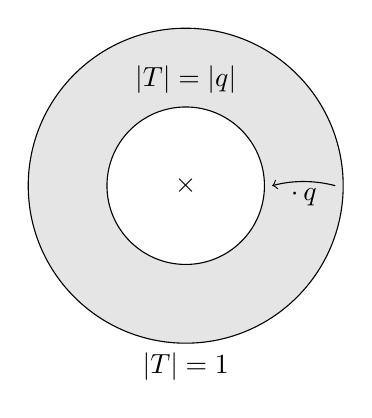
\begin{tikzpicture}[scale=1.0]
  \fill [black!10, even odd rule] (0, 0) circle[radius=2] circle[radius=1];
  \draw (0,0) circle (2);
  \draw (0,0) circle (1);
  \node at (0,0) {$\times$};
  \node[below] at (0,-2) {$|T|=1$};
  \node[above] at (0.0,1.05) {$|T|=|q|$};
  \draw[->] (1.9,0) arc (75:105:1.55);
  \node at (1.5,-0.15) {$\cdot\,q$};
\end{tikzpicture}
\end{center}

\begin{remark}[$E_q$ is algebraic]
\label{rmk:12:algebraic}
$E_q$ is proper (it is compact, obtained from the compact annulus by gluing),
separated, and smooth (locally it is just $\Gm^{\mathrm{an}}$), hence a proper
smooth connected curve of relative dimension $1$ over $\mathbb{Z}(\!(q)\!)$. In
any reasonable analytic geometry a proper smooth curve is automatically
algebraic: the inverse of the ideal sheaf of a closed point (e.g. the identity
section, which exists here) is an ample line bundle, and a Riemann--Roch type
statement then produces enough functions to embed it. Thus $E_q$ is the
analytification of an honest elliptic curve over the abstract ring
$\mathbb{Z}(\!(q)\!)$.
\begin{equation*}
E_q\ \text{is a proper smooth curve over } \mathbb{Z}(\!(q)\!),\ \text{hence an elliptic curve.}
\end{equation*}
Scholze noted that the global algebraicity in this argument implicitly uses a
GAGA statement over a nice noetherian base, and that over a more general base
$\Spa$ of a Huber pair the passage from a local (formal-model) ample bundle to a
global one is not obviously automatic; here the identity section makes it work.
\end{remark}

\begin{proposition}[Weierstrass equation]
\label{prop:12:weierstrass}
Removing the origin, $E_q$ has the Weierstrass form
\begin{equation*}
E_q\setminus\{0\}:\qquad y^{2}+xy\ =\ x^{3}-a_{4}x-a_{6},
\end{equation*}
where (having inverted $2$ to eliminate one term)
\begin{equation*}
a_{4}\ =\ \sum_{n\ge 1} 5\,n^{3}\,\frac{q^{n}}{1-q^{n}},
\qquad
a_{6}\ =\ \sum_{n\ge 1}\frac{7n^{5}+5n^{3}}{12}\,\frac{q^{n}}{1-q^{n}}
\end{equation*}
are power series in $q$.\footnote{Copied by Scholze from Wikipedia. The board
index reads $n\ge 0$, but the $n=0$ term is ill-defined, so the intended range
is $n\ge 1$. With that range these are the standard Tate-curve coefficients:
writing $s_k(q)=\sum_{n\ge1}\tfrac{n^k q^n}{1-q^n}$, one has $a_4=5s_3(q)$ and
$a_6=\tfrac{7s_5(q)+5s_3(q)}{12}$, so that
$y^2+xy=x^3-5s_3\,x-\tfrac{5s_3+7s_5}{12}$ (cf. Silverman, \emph{Advanced Topics
in the Arithmetic of Elliptic Curves}, Ch.~V).}
\end{proposition}

\begin{remark}[Polynomial growth of the coefficients]
\label{rmk:12:polynomial-growth}
Expanding $\tfrac{1}{1-q^{n}}=1+q^{n}+q^{2n}+\cdots$ and collecting, one may
write $a_{4}=\sum_{N} c_{N}q^{N}$ (and likewise $a_6$); what struck Scholze on
first seeing these formulas is that the resulting coefficients $c_N$ have at
worst \emph{polynomial} growth in $N$. This has two consequences.
\begin{itemize}
\item One may specialise $q$ to any $q\in\mathbb{C}$ with $0<|q|<1$, obtaining an
actual complex torus $\mathbb{C}^{\ast}/q^{\mathbb{Z}}$; the analytic description
$\Gm/q^{\mathbb{Z}}$ makes literal sense there. So the formal object
specialises to any intermediate radius, not just to a formal neighbourhood.
\item Convergence for $0<|q|<1$ is equivalent to \emph{subexponential} growth of
the coefficients:
\begin{equation*}
\text{convergence for } 0<|q|<1\quad\Longleftrightarrow\quad
\text{subexponential growth of coefficients.}
\end{equation*}
\end{itemize}
Polynomial growth is strictly stronger than subexponential. There is a clear
geometric reason the coefficients must grow subexponentially (the curve is
defined over the open unit disk), but it is not clear how to see the sharper
polynomial bound geometrically. Pinning down the smallest ring over which $E_q$
lives --- one enforcing polynomial growth --- is exactly what the ``gaseous''
structure of \cref{thm:12:gaseous} will achieve.
\end{remark}

\subsection{Berkovich spectra and the geometry of \texorpdfstring{$\mathbb{Z}(\!(q)\!)$}{Z((q))}}

We now study the geometry of $\Spa(\mathbb{Z}(\!(q)\!),\mathbb{Z}[\![q]\!])$,
the adic spectrum of continuous valuations. The topologically nilpotent unit
$q$ is a convenient handle: it lets one gauge the size of any function by
comparison with $|q|$. In particular there is a unique order-preserving
$|q|\mapsto\tfrac12$ map $\Gamma\cup\{0\}\to\mathbb{R}_{\ge0}$ out of the value
group, so each continuous valuation acquires a real-valued absolute value. For
most valuations this is injective, the exception being certain rank-$2$
valuations carrying a little extra infinitesimal information not remembered by
the real value. This gives a comparison map to the Berkovich spectrum.

\begin{definition}[Berkovich spectrum]
\label{def:12:berkovich}
For a Banach ring $R$, the \emph{Berkovich spectrum} is
\begin{equation*}
\MBerk(R)\ =\ \Bigl\{\,|\cdot|\colon R\to\mathbb{R}_{\ge0}\ \Big|\
|0|=0,\ |1|=1,\ |xy|=|x||y|,\ |x+y|\le|x|+|y|,\ |x|\le\|x\|_R\,\Bigr\},
\end{equation*}
the set of multiplicative seminorms bounded by the Banach norm $\|\cdot\|_R$,
topologised as a subspace of $\prod_{x\in R}[0,\|x\|_R]$. Since each factor is a
compact interval and all the defining conditions are closed, $\MBerk(R)$ is a
compact Hausdorff space.
\end{definition}

Note that Berkovich allows the ordinary triangle inequality $|x+y|\le|x|+|y|$,
not only the strong (nonarchimedean) one, so the theory is not restricted to the
nonarchimedean setting.

\begin{proposition}[Adic spectrum as maximal Hausdorff quotient]
\label{prop:12:spa-berk}
The comparison map
\begin{equation*}
\Spa\bigl(\mathbb{Z}(\!(q)\!),\mathbb{Z}[\![q]\!]\bigr)\ \longrightarrow\
\MBerk\bigl(\mathbb{Z}(\!(q)\!)\bigr)
\end{equation*}
exhibits the target as the \emph{maximal Hausdorff quotient} of the source. The
only difference between the two is the presence of higher-rank valuations in the
adic spectrum, which produce very infinitesimal changes; up to those, the two
spaces coincide.
\end{proposition}

The base of both spaces is the Berkovich spectrum of $\mathbb{Z}$, which --- in
contrast to the nearly point-like scheme-theoretic spectrum --- is a genuinely
interesting space. Here $\mathbb{Z}$ carries the norm with $\|0\|_{\mathbb{Z}}=0$
and $\|n\|_{\mathbb{Z}}=1$ for $n\ne0$ (every integer lies in the unit ball), the
nonarchimedean choice.

\begin{proposition}[$\MBerk(\mathbb{Z})$]
\label{prop:12:berkovich-Z}
With the norm $\|n\|_{\mathbb{Z}}\in\{0,1\}$, the Berkovich spectrum
$\MBerk(\mathbb{Z})$ is a tree: a generic point (the trivial, ``$0$-or-$1$'',
absolute value) from which, for each prime $p$, a ray emanates --- an interval
of $p$-adic absolute values $\|\cdot\|_p^{\alpha}$, $\alpha\in(0,\infty)$ ---
ending at a closed point $\mathbb{F}_p$ (the trivial absolute value on
$\mathbb{F}_p$). The points correspond to maps to complete Banach fields:
\begin{equation*}
\mathbb{Q}\ (\text{trivial abs. value}),\qquad
\mathbb{Q}_p\ (\text{abs. value with } |p|\in(0,1)),\qquad
\mathbb{F}_p\ (\text{trivial abs. value}).
\end{equation*}
\end{proposition}

% board 7 @ 00:41:12 --- tree M^Berk(Z): generic trivial-norm point, one ray per prime ending at F_p
\begin{center}
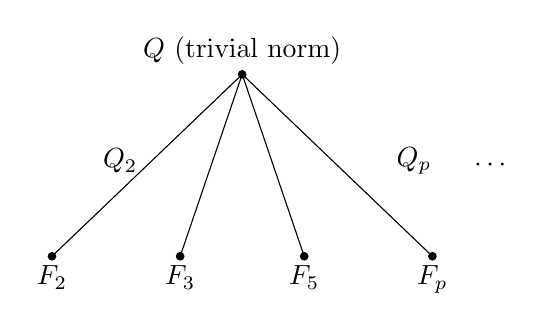
\begin{tikzpicture}[scale=1.05]
  \coordinate (top) at (0,2.2);
  \coordinate (f2) at (-2.3,0);
  \coordinate (f3) at (-0.75,0);
  \coordinate (f5) at (0.75,0);
  \coordinate (fp) at (2.3,0);
  \draw (top) -- (f2);
  \draw (top) -- (f3);
  \draw (top) -- (f5);
  \draw (top) -- (fp);
  \fill (top) circle (1.5pt);
  \fill (f2) circle (1.5pt);
  \fill (f3) circle (1.5pt);
  \fill (f5) circle (1.5pt);
  \fill (fp) circle (1.5pt);
  \node[above] at (top) {$\mathbb{Q}$ (trivial norm)};
  \node[below] at (f2) {$\mathbb{F}_2$};
  \node[below] at (f3) {$\mathbb{F}_3$};
  \node[below] at (f5) {$\mathbb{F}_5$};
  \node[below] at (fp) {$\mathbb{F}_p$};
  \node[left] at (-1.15,1.15) {$\mathbb{Q}_2$};
  \node[right] at (1.75,1.15) {$\mathbb{Q}_p$};
  \node at (3.0,1.1) {$\cdots$};
\end{tikzpicture}
\end{center}

\begin{remark}[Fibres over $\MBerk(\mathbb{Z})$]
\label{rmk:12:fibres}
The space $\MBerk(\mathbb{Z}(\!(q)\!))$ fibres over $\MBerk(\mathbb{Z})$, and one
can describe the fibres. The statement is essentially Ostrowski's theorem, which
determines the multiplicative seminorms once $|q|$ is fixed.
\begin{itemize}
\item Over the closed point $\mathbb{F}_p$, the fibre is a single point: the base
change is $\mathbb{F}_p(\!(q)\!)$, already a nonarchimedean field with $|q|$
fixed to $\tfrac12$.
\item Over the ray of $\mathbb{Q}_p$-absolute values, the fibre is a
\emph{punctured open unit disk over $\mathbb{Q}_p$}. The map to the ray is a
radius map. Its generic point is $\mathbb{Q}(\!(q)\!)$; the fibre over a fixed
point on the ray is an annulus (a locus where $|q|$ is fixed).
\end{itemize}
Geometrically, $\MBerk(\mathbb{Z}(\!(q)\!))$ has one punctured open unit disk for
each place; the pieces are glued so that moving \emph{towards the centre} of a
disk lands at the common generic point $\mathbb{Q}(\!(q)\!)$, while moving
\emph{towards the boundary} lands at the corresponding $\mathbb{F}_p(\!(q)\!)$.
Thus $\mathbb{F}_p(\!(q)\!)$ sits near the boundary of the annulus, and as one
moves inward along the ray towards $\mathbb{Q}$ the annuli move towards the
origin.
\end{remark}

\subsection{An archimedean variant of \texorpdfstring{$\mathbb{Z}(\!(q)\!)$}{Z((q))}}

The tree picture suggests enlarging $\MBerk(\mathbb{Z})$ by allowing the
\emph{usual} archimedean norm on $\mathbb{Z}$ in addition to the nonarchimedean
one. Then, besides the $p$-adic rays, there is an archimedean ray
\begin{equation*}
\mathbb{Z}\to\mathbb{R}\xrightarrow{\ |\cdot|^{\alpha}\ }\mathbb{R}_{\ge0},
\qquad \alpha\in(0,1],
\end{equation*}
where $|\cdot|$ is the usual absolute value of $\mathbb{R}$. Unlike the
$p$-adic rays (parametrised by $\alpha\in(0,\infty)$), the archimedean ray stops
at $\alpha=1$: raising the usual absolute value to a power $\alpha>1$ violates
the triangle inequality. So the real place ``stops in the middle'' compared to
the others.

\begin{definition}[The Banach ring $\mathbb{Z}(\!(q)\!)_{1/2}$]
\label{def:12:Zq-half}
Endow the ring $\mathbb{Z}[q^{\pm1}]$ with the norm
\begin{equation*}
\Bigl|\,\sum_{n\in\mathbb{Z}} a_n q^{n}\,\Bigr|\ =\ \sum_{n}|a_n|\,\tfrac{1}{2^{n}}
\end{equation*}
(usual absolute value on $\mathbb{Z}$, and $|q|=\tfrac12$) and complete it to a
Banach ring
\begin{equation*}
\mathbb{Z}(\!(q)\!)_{1/2}\ =\ \Bigl\{\,f=\sum_n a_n q^{n}\ \Big|\
\sum_n |a_n|\,\tfrac{1}{2^{n}}<\infty\,\Bigr\}.
\end{equation*}
Its elements converge for $q\in\mathbb{C}$ with $0<|q|\le\tfrac12$, and each
defines a holomorphic function of $q$ on that region, continuous up to the
boundary.
\end{definition}

The Berkovich spectrum $\MBerk(\mathbb{Z}(\!(q)\!)_{1/2})$ has, at its
archimedean part, a genuinely complex-analytic piece: the disk
\begin{equation*}
\bigl\{\,q\in\mathbb{C}\ \big|\ 0<|q|\le\tfrac12\,\bigr\}\big/\Gal(\mathbb{C}/\mathbb{R})
\ \longrightarrow\ \MBerk\bigl(\mathbb{Z}(\!(q)\!)_{1/2}\bigr),
\end{equation*}
where one quotients by complex conjugation because conjugate values give the
same absolute value. This is the picture in which one would like to combine
archimedean and nonarchimedean geometry: parts of the space are literally
real- or complex-analytic, others nonarchimedean, all inside one space. The one
awkward feature is that fixing $|q|=\tfrac12$ makes the archimedean punctured
disk stop at radius $\tfrac12$, although from the point of view of the Tate curve
there was no reason to stop before $|q|=1$.

\subsection{Free complete modules, and the liquid structure}

\begin{remark}[The question, and the answer]
\label{rmk:12:liquid-question}
Can one endow $\mathbb{Z}(\!(q)\!)_{1/2}$ with a natural analytic ring structure?
The answer is yes: the \emph{liquid} analytic ring structure
\cite{clausen2020analytic}. It is slightly better to work with
\begin{equation*}
\mathbb{Z}(\!(q)\!)_{>1/2}\ =\ \bigcup_{r>1/2}\mathbb{Z}(\!(q)\!)_{r},
\end{equation*}
functions converging on some disk of radius slightly larger than $\tfrac12$.
This is Scholze's answer to question~(2) of \cref{rmk:12:two-questions}: the
liquid structure combines the archimedean and nonarchimedean settings. This was
very much on Clausen and Scholze's minds when they first found the solid theory
and tried to go further; the eventual answer was the liquid construction.
\end{remark}

The 2019 mindset for producing an analytic ring structure is to \emph{describe
the free complete modules}. For a light profinite set $S=\varprojlim_i S_i\in
\ProFin_{\mathbb{N}}(\mathrm{Fin})$ we compare three descriptions of the free
module.

\begin{example}[Solid and abstract free modules]
\label{ex:12:free-solid-abstract}
For $S=\varprojlim_i S_i$:
\begin{enumerate}
\item The \emph{solid} free module is the inverse limit
\begin{equation*}
\mathbb{Z}[S]^{\solid}\ \xrightarrow{\ \sim\ }\ \varprojlim_i \mathbb{Z}[S_i]
\ =\ \iHom\bigl(\Cont(S,\mathbb{Z}),\mathbb{Z}\bigr),
\end{equation*}
the $\mathbb{Z}$-valued measures on $S$ (\cref{rmk:5:measures}): a measure assigns
an integer to each clopen subset, additively.
\item The \emph{abstract} (uncompleted) free module sits inside it as the
$\ell^{0}$-bounded part,
\begin{equation}
\label{eq:12:free-abstract}
\mathbb{Z}[S]\ \xrightarrow{\ \cong\ }\
\bigcup_{n>0}\ \varprojlim_i\ \mathbb{Z}[S_i]_{\ell^{0}\le n},
\end{equation}
where $\mathbb{Z}[S_i]_{\ell^{0}\le n}$ consists of the sums of at most $n$ basis
elements (with multiplicity). Here Scholze's $\ell^{0}$-norm counts the total
number of basis vectors used; on a discrete finite free group it agrees with
$\ell^{1}$, but he prefers to call it $\ell^{0}$.
\end{enumerate}
\end{example}

The liquid free module is a third possibility, interpolating between the
uncompleted and solid ones by a convergence (norm) condition.

\begin{definition}[Liquid free module]
\label{def:12:liquid-free}
Endow each $\mathbb{Z}(\!(q)\!)_{r}[S_i]$ with the norm
\begin{equation*}
\Bigl\|\ \sum_{\substack{n\in\mathbb{Z}\\ s\in S_i}} a_{n,s}\,q^{n}[s]\ \Bigr\|
\ =\ \sum_{n,s}\|a_{n,s}\|\,r^{n}.
\end{equation*}
Then the free liquid module on $S$ over $\mathbb{Z}(\!(q)\!)_{>1/2}$ is
\begin{equation}
\label{eq:12:liquid-free}
\mathbb{Z}(\!(q)\!)_{>1/2}[S]^{\mathrm{liq}_q}\ =\
\bigcup_{r>1/2}\ \bigcup_{c>0}\ \varprojlim_i\
\mathbb{Z}(\!(q)\!)_{r}[S_i]_{\|\cdot\|\le c}.
\end{equation}
Once the radius $r$ and the size bound $c$ are fixed, the inverse limit of the
bounded parts is compact Hausdorff, so the whole is a well-behaved condensed
set. The hard theorem \cite{clausen2020analytic} is that this proposal really
satisfies the axioms of an analytic ring; the description
\eqref{eq:12:liquid-free} is what suggests itself as soon as one asks for a
notion of complete module over this Banach ring.
\end{definition}

\subsection{Analytic ring structures on \texorpdfstring{$\mathbb{R}$}{R}}

Answering question~(1) of \cref{rmk:12:two-questions}, one specialises the liquid
ring to the reals. Send $q\mapsto t$ with $0<t<\tfrac12$; the map
$\mathbb{Z}(\!(q)\!)_{>1/2}\to\mathbb{R}$ defines a point of the archimedean
Berkovich space lying over $\MBerk(\mathbb{Z})$, hence over some power
$|\cdot|^{\alpha}$ of the usual absolute value of $\mathbb{R}$. The value of $t$
determines $\alpha\in(0,1]$ by the relation
\begin{equation*}
t^{\alpha}=\tfrac12,
\end{equation*}
whose meaning is precisely that the point maps to the parameter $\alpha$ on the
archimedean ray of $\MBerk(\mathbb{Z})$.

\begin{definition}[$\alpha$-liquid ring structure on $\mathbb{R}$]
\label{def:12:alpha-liquid-R}
For $0<\alpha\le1$ one obtains the \emph{$\alpha$-liquid} analytic ring structure
on $\mathbb{R}$, whose complete modules are forced by requiring completeness only
after forgetting the linear structure. Its free modules are
\begin{equation}
\label{eq:12:R-alpha-liquid}
\mathbb{R}[S]^{\alpha\text{-}\mathrm{liq}}\ =\
\bigcup_{\beta<\alpha}\ \bigcup_{c>0}\ \varprojlim_i\
\mathbb{R}[S_i]_{\ell^{\beta}\le c},
\qquad
\Bigl\|\ \sum_i x_i[s_i]\ \Bigr\|_{\ell^{\beta}}\ =\ \sum_i |x_i|^{\beta},
\quad 0<\beta<1.
\end{equation}
The union over $\beta<\alpha$ is filtered, the bounded loci
$\{\|\cdot\|_{\ell^\beta}\le c\}$ growing as $\beta$ increases.
\end{definition}

\begin{remark}[Non-local convexity]
\label{rmk:12:non-locally-convex}
For $0<\beta<1$ the quantity $\|\cdot\|_{\ell^\beta}$ satisfies the triangle
inequality but not the usual scaling axiom of a norm (it scales by the
$\beta$-th power); it is not a norm in the standard sense. The $\ell^\beta$
``balls'' are \emph{not convex}: in two dimensions the unit ball is a
four-pointed concave star. These $\ell^\beta$ with $\beta<1$ sit to the left of
the usual locally convex $\ell^p$ ($1\le p\le\infty$), and the liquid theory is
forced to use such non-locally-convex spaces.
\end{remark}

% board 17 @ 01:25:53 --- non-convex unit ball of the ell^beta "norm", 0<beta<1
\begin{center}
\begin{tikzpicture}[scale=1.2]
  \draw (1,0) .. controls (0.18,0.18) .. (0,1)
              .. controls (-0.18,0.18) .. (-1,0)
              .. controls (-0.18,-0.18) .. (0,-1)
              .. controls (0.18,-0.18) .. (1,0);
  \draw[->] (-1.35,0) -- (1.45,0);
  \draw[->] (0,-1.35) -- (0,1.45);
\end{tikzpicture}
\end{center}

\begin{remark}[Warning: Radon measures do not work]
\label{rmk:12:radon-warning}
The naive guess is that the complete modules over $\mathbb{R}$ should be the
Radon measures, i.e. that the free module should be
\begin{equation*}
\mathbb{R}[S]^{\wedge}\ :=\ \MRadon(S)\ =\ \iHom\bigl(\Cont(S,\mathbb{R}),\mathbb{R}\bigr).
\end{equation*}
This \emph{does not} define an analytic ring structure. The reason is that
complete modules must be stable under extensions, and locally convex
topological vector spaces are not: there is a natural extension of a Banach space
by $\mathbb{R}$ (a one-dimensional space) --- i.e. with $\mathbb{R}$ as the
subspace --- whose total space is not locally convex. Scholze attributed this
three-space phenomenon to Ribe, arising from the entropy functional; it is a
meaningful object, not a pathology, but it destroys the Radon-measure
option.\footnote{The transcript's date (``around 1918'') is certainly a
mishearing. The non-locally-convex three-space example is due to M.~Ribe,
\emph{Examples for the nonlocally convex three space problem}, Proc.\ Amer.\
Math.\ Soc.\ \textbf{73} (1979), 351--355: a nontrivial twisted sum
$0\to\mathbb{R}\to X\to\ell^1\to 0$ built from the entropy function
$t\mapsto t\log t$. The general twisted-sum method is due to Kalton--Peck (1979).}
Once one
allows non-locally-convex spaces into the picture the theory works again --- but
one is forced into them.
\end{remark}

The naive Radon-measure structure is really the opposite endpoint: taking the
$\ell^{1}$ (locally convex) construction reproduces the Radon measures, which are
related to the classical theory of complete locally convex complex vector spaces
in the same way that solid modules are related to the classical theory of
complete (pro-discrete) modules.

\subsection{Analytic ring structures on \texorpdfstring{$\mathbb{Q}_p$}{Qp}}

One may instead specialise $\mathbb{Z}(\!(q)\!)_{>1/2}\to\mathbb{Q}_p$. Naively
one might expect nothing new at the nonarchimedean places --- that the extra
archimedean convergence condition is invisible there and one simply recovers the
solid structure. This is false: one gets genuinely new structures.

\begin{definition}[$\alpha$-liquid ring structure on $\mathbb{Q}_p$]
\label{def:12:alpha-liquid-Qp}
Specialising to $\mathbb{Q}_p$ (sending $q$ to a suitable power of $p$, so that
any $\alpha$ is allowed), one obtains for every $0<\alpha<\infty$ --- i.e. for
every point of the $p$-adic ray of $\MBerk(\mathbb{Z})$ --- an
\emph{$\alpha$-liquid} analytic ring structure on $\mathbb{Q}_p$, with free
modules
\begin{equation*}
\mathbb{Q}_p[S]^{\alpha\text{-}\mathrm{liq}}\ =\
\bigcup_{\beta<\alpha}\ \bigcup_{c>0}\ \varprojlim_i\
\mathbb{Q}_p[S_i]_{\ell^{\beta}\le c},
\end{equation*}
using the $\ell^{\beta}$-norm of \eqref{eq:12:R-alpha-liquid}. This should be
compared with the solidification, which is the $\ell^{\infty}$ (i.e.
$\alpha=\infty$) endpoint:
\begin{equation*}
\mathbb{Q}_p[S]^{\solid}\ =\ \bigcup_{c>0}\ \varprojlim_i\
\mathbb{Q}_p[S_i]_{\ell^{\infty}\le c}.
\end{equation*}
\end{definition}

So even over $\mathbb{Q}_p$, where the solid theory already worked well, there is
a whole new world of analytic ring structures, one for each $\alpha\in(0,\infty)$.

\subsection{The spectrum of structures, and the gaseous ring}

\begin{remark}[Solid, liquid, gaseous]
\label{rmk:12:states-of-matter}
The various structures organise into a family parametrised by
$\alpha\in[0,\infty]$:
\begin{equation}
\label{eq:12:spectrum-interval}
\underset{\text{all condensed modules}}{\text{gaseous}\ (0)}
\ \cdots\ \underset{\alpha}{\alpha\text{-liquid}}\ \cdots\
\underset{\infty}{\text{solid}}.
\end{equation}
The class of complete modules \emph{grows} as $\alpha$ decreases: being solid is
a much stricter condition than being $\alpha$-liquid. At the endpoint $\alpha=0$
one recovers \emph{all} condensed modules --- a naive $\ell^{0}$-condition (a
bound on the number of nonzero coefficients) reproduces all condensed modules,
by a variant of the description in \eqref{eq:12:free-abstract}. The three regimes
are Scholze's ``solid / liquid / gaseous'' states of matter.
\end{remark}

% board 20 @ 01:32:01 --- the interval of structures from gaseous (0) through alpha-liquid to solid
\begin{center}
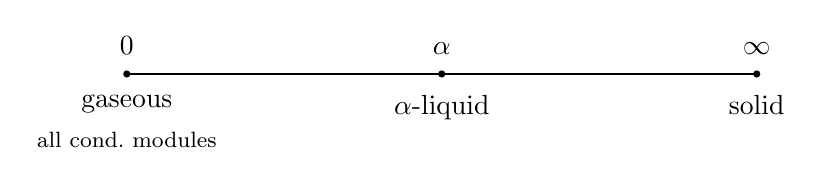
\begin{tikzpicture}[scale=1.0]
  \draw (0,0) -- (8,0);
  \fill (0,0) circle (1.3pt);
  \fill (4,0) circle (1.3pt);
  \fill (8,0) circle (1.3pt);
  \node[above] at (0,0.12) {$0$};
  \node[above] at (4,0.12) {$\alpha$};
  \node[above] at (8,0.12) {$\infty$};
  \node[below] at (0,-0.15) {gaseous};
  \node[below] at (0,-0.62) {\footnotesize all cond.\ modules};
  \node[below] at (4,-0.15) {$\alpha$-liquid};
  \node[below] at (8,-0.15) {solid};
\end{tikzpicture}
\end{center}

\begin{remark}[The course's method: impose endomorphisms of $P$]
\label{rmk:12:mindset-endomorphisms}
The 2019 mindset (describe the free complete modules, then prove the axioms by
hand) is replaced in this course by a lighter method. To define an analytic ring
structure one instead finds natural endomorphisms of the compact projective
generator
\begin{equation*}
P\ =\ A[\mathbb{N}\cup\{\infty\}]\big/[\infty]
\end{equation*}
--- the free complete module on a null sequence --- that one \emph{wants} to
become isomorphisms. Because in light condensed abelian groups $P$ is compact and
internally projective (\cref{thm:3:three-properties,def:5:solid}), imposing such
isomorphisms automatically defines an analytic ring structure. This makes new
structures very easy to produce.
\end{remark}

\begin{remark}[What the Tate curve needs]
\label{rmk:12:tate-needs-two}
To carry out the construction of the Tate elliptic curve one needs only two
properties, both with a clear meaning in terms of the underlying condensed ring:
\begin{enumerate}
\item $q$ is a topologically nilpotent unit --- i.e. the map from the free ring
on a null sequence, sending the generator $1\mapsto q$, is available; and
\item $1-q\cdot\mathrm{shift}\colon P\to P$ is an isomorphism.
\end{enumerate}
There is an evident universal (initial) example: take the free ring on a
topologically nilpotent unit and impose~(2).
\end{remark}

\begin{theorem}[The gaseous analytic ring]
\label{thm:12:gaseous}
There is an initial analytic ring $A=(\ur A,\Mod_A)$ with a topologically
nilpotent unit $q$ and with $1-q\cdot\mathrm{shift}$ an automorphism of $P$ ---
the \emph{gaseous} analytic ring structure. Its underlying ring is the ring of
Laurent series with polynomially bounded coefficients,
\begin{equation}
\label{eq:12:gaseous-underlying}
\ur A(\ast)\ =\ \Bigl\{\,\sum_n a_n q^{n}\in\mathbb{Z}(\!(q)\!)\ \Big|\
(a_n)\ \text{has at most polynomial growth}\,\Bigr\},
\end{equation}
and its free modules on $S=\varprojlim_i S_i$ are
\begin{equation}
\label{eq:12:gaseous-free}
A[S]\ =\ \bigcup_{k>0}\ \bigcup_{n>0}\ \varprojlim_i\ \mathbb{Z}(\!(q)\!)[S_i],
\end{equation}
where the coefficient of $q^{m}$ is required to have $\ell^{0}$-norm at most
$m+m^{k}$ (polynomial growth of degree $k$ in the exponent $m$, the summand $m$
allowing negative Fourier coefficients).\footnote{Scholze wavered between
$\ell^{0}$ and $\ell^{1}$ for the per-degree bound; the board reads $\ell^{0}$,
and on a discrete free module the two agree (\cref{ex:12:free-solid-abstract}),
so the distinction is immaterial here. The precise description, deferred at this
point, is worked out in \cref{lec:14}: there the coefficient of $q^{m}$ is
required to lie in the $\ell^{1}$-ball $\mathbb{Z}[S_i]_{\le(n+m)^{k}}$
(\cref{thm:14:gaseous-base}).}
\end{theorem}

\begin{remark}[The Tate curve over the smallest ring]
\label{rmk:12:tate-over-gaseous}
Doing analytic geometry over the gaseous ring, one can repeat the construction of
the Tate curve and see, for geometric reasons, that it lives over exactly this
smallest ring \eqref{eq:12:gaseous-underlying} --- the one enforcing the
polynomial growth observed in \cref{rmk:12:polynomial-growth}, rather than merely
subexponential growth. Specialising back, the gaseous analytic ring sits close
to, but not quite at, the $\alpha=0$ end of the spectrum
\eqref{eq:12:spectrum-interval}. Base change of the free-module description
\eqref{eq:12:gaseous-free} to $\mathbb{Q}_p$ is a somewhat nasty but instructive
exercise, left for a future lecture.
\end{remark}
